\chapter{Combination Logic Design}

\section{Introduction}
A \textbf{circuit} is a network that processes distinct-value variables. It has:
\begin{itemize}
    \item one or more input terminals
    \item one or more output terminals
    \item a functional specification (expressed by a truth table)
    \item a timing specification
\end{itemize}
Digital circuits are classified as \textbf{sequential} or \textbf{combinational} (this chapter will discuss the later one). The difference
between these two is, that a combinational circuit combines the current input values to compute the output, whereas in a sequential circuit,
the output depends on the current input and on the previous input values. In another way, a combinational circuit is \textbf{memoryless} and 
a sequential circuit has \textbf{memory}.

Combination circuit therefore have to satisfie the following requirements:
\begin{itemize}
    \item every circuit (element) is itself combinational
    \item every wire (node) of the circuit is either designated as input or output
    \item the circuit contains no cyclic paths
\end{itemize}

\section{Boolean Algebra}

\begin{definition}
    \begin{itemize}
        \item \textbf{Complement} - The inverse of a variable, $\bar{A}$
        \item \textbf{Literal} - A variable in a equation
        \item \textbf{Product} - The AND of two or more literals
        \item \textbf{Minterm} - The product of all inputs (or their complement) of a function
        \item \textbf{Sum} - The OR of two or more literals
        \item \textbf{Maxterm} - The sum of all inverse of inputs (or their complement) of a function
        \item \textbf{Precedence} - The order of operations: NOT > AND > OR
        \item \textbf{Sum of product form (SOP)} - The sum of all minterms for which a function is true
        \item \textbf{Product of sum form (POS)} - The product of all maxterms for which a function is false
        \item \textbf{Prime implication} - An implicant that cannot be combined with other implicants to for a new implicant with fewer literals
    \end{itemize}
\end{definition}

\subsection{Axioms and Theorems}

\begin{figure}[h]
    \centering
    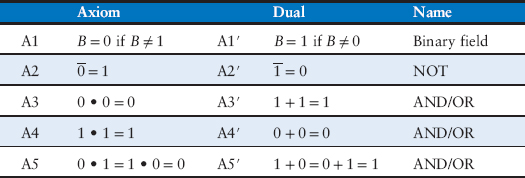
\includegraphics[width=10cm]{axiom.jpg}
    \caption{Axioms}
\end{figure}

\begin{figure}[h]
    \centering
    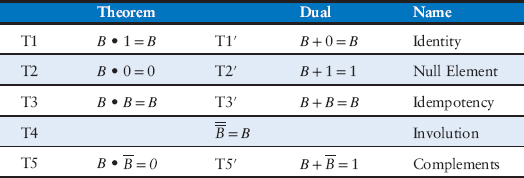
\includegraphics[width=10cm]{theorem.jpg}
    \caption{Theorems}
\end{figure}

\begin{figure}[h]
    \centering
    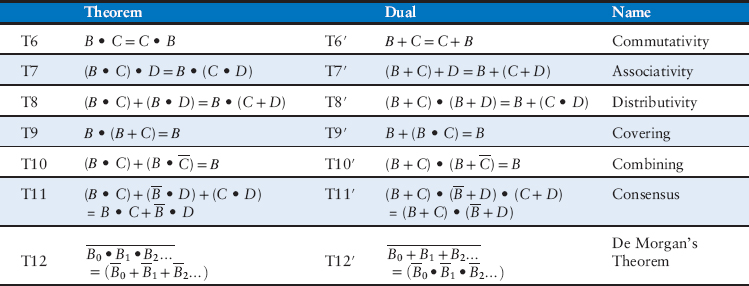
\includegraphics[width=10cm]{theorem multiple.jpg}
    \caption{Theorems for multiple variables}
\end{figure}

\pagebreak
We can use these helpful theorems to reduce boolean equations into prime implicants.

\section{From Logic to Gates}
When drawing a \textbf{schemantic} we generally follow these rules:
\begin{itemize}
    \item Inputs are on the left / top side
    \item Ouputs are on the right / bottom side
    \item Gates should flow from left to right
    \item Straight wires are better
    \item Wires always connect at a T Junction
    \item Wires crossing without a dot make no connection
\end{itemize}
To draw such a schemantic it can be usefull to first draw a truth table. In a truth table a X marks 
a don't care.

\section{Multilevel Combinational Logic}
In this section we will shortly mention bubble pushing as a helpful way to redraw combinational 
circuits so that bubbles cancle out and the function can be more easily determined. (More details 
can be found in the book)

\section{Illegal and Floating Values}
The symbol X indicates that the circuit node has an \textbf{unknown} or \textbf{illegal} value, this 
commonly happens if a node is being driven both by a 0 and a 1 at the same time. This situation is 
also called \textbf{contention}. Be carefull to not mistake this X with a don't care in truth tables.

The symbol Z denotes that a node is being driven neither by HIGH nor LOW. The node is said to be 
\textbf{floating, heigh impedance} or \textbf{high Z}. In reality, a floating node might be 0 or 1 
or something in between.

\section{Karnaugh Maps}
Karnaugh Maps are a usefull graphical method for simplifying Boolean equations. They work well for 
equations with up to four variables. 

\begin{figure}[h]
    \centering
    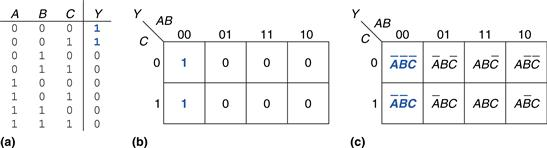
\includegraphics[width=13cm]{karnaugh.jpg}
    \caption{A Karnaugh Maps}
\end{figure}

Note that the AB combinations are in Gray code.

\begin{figure}[h]
    \centering
    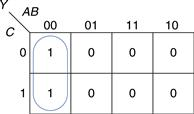
\includegraphics[width=6cm]{karnaugh2.jpg}
    \caption{A Karnaugh Maps}
\end{figure}

We use the following rules to minimize a expression using a K-map:
\begin{itemize}
    \item Us the fewest circles necessary to cover all 1's
    \item A circle can only contain 1's
    \item Each circle must span a rectangular block that is a power of 2 in each direction
    \item Each circle should be as large as possible
    \item A circle may wrap around the edge of the K-map
    \item A 1 in a K-map may be circled multiple times
\end{itemize}

\section{Combinational Building Blocks}
Combinational Logic is often grouped into larger building blocks to build more complex systems. This is an application fo the
principle of abstraction. Some of these building blocks are full adders, priority circuits and seven-segment display decoders.
In this section we will look at another two building blocks.

\subsection{Multiplexer (mux)}

Multiplexers (short mux) are among the most commonly used combinational circuits. They choose an output among 
several possible inputs based on the value of a select signal. A 2:1 mux chooses between 2 different input signals.

\begin{figure}[h]
    \centering
    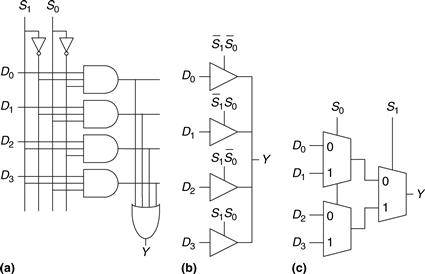
\includegraphics[width=11cm]{mux.jpg}
    \caption{4:1 mux implementations}
\end{figure}

\subsection{Decoders}
A decoder has $n$ inputs and $2^n$ outputs. It asserts exactly one of its outputs depending on the input combination.
The output of a decoder are called \textbf{one-hot}, because exactly one of them is hot at a given time.

\begin{figure}[h]
    \centering
    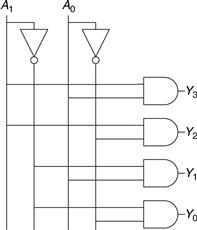
\includegraphics[width=6cm]{decoder.jpg}
    \caption{2:4 decoder}
\end{figure}

\pagebreak
\section{Timing}
An output takes time to change in response to a change of input. We can draw a \textbf{timing diagram} to visialize the
transient response of a combinational circuit. The transition from LOW to HIGH is called the \textbf{rising edge} and from HIGH
to LOW it's called the \textbf{falling edge}. 

\begin{figure}[h]
    \centering
    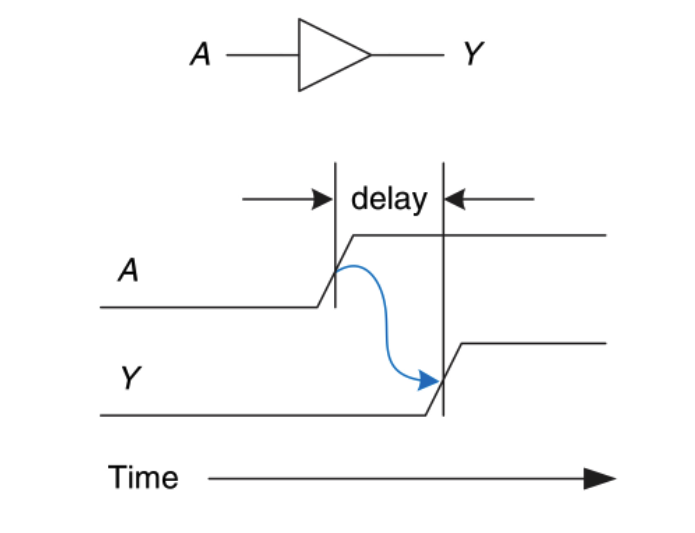
\includegraphics[width=10cm]{timing.png}
    \caption{timing diagram of a buffer}
\end{figure}

Combinational logic is characterized by its \textbf{propagation delay $t_{pd}$}, the maximum time from when a input changes
until the output reaches their final state, and the \textbf{contamination delay $t_{cd}$}, the minimum time from an input 
change until the output starts changing.

Since $t_{pd}$ and $t_{cd}$ are determined by signal paths in a combinational circuit, we introduce the following two 
definitions:

\begin{itemize}
    \item \textbf{Critical path} - The longest and therefore slowest path in a circuit
    \item \textbf{Shortest path} - The shortest and therefore fastest path through a circuit
\end{itemize}

We can now calculate the $t_{pd}$ by adding up the propagation time for each element along the critical path, and similarly calculate 
the $t_{cp}$ by adding all propagation times along the short path.